\ifx\allfiles\undefined
\documentclass[12pt, a4paper, oneside, UTF8]{ctexbook}
\def\path{../config}
\input{\path/package.tex}

% 定理环境设置
\input{\path/theorem1_zh.tex}

\input{\path/custom.tex}

% 修改参数改变封面样式，0 默认原始封面、内置其他1、2、3种封面样式
\def\myIndex{3}


\ifnum\myIndex>0
    \input{\path/cover_package_\myIndex} 
\fi

\def\myTitle{高等数学笔记}
\def\myAuthor{M.K.}
\def\myDateCover{\today}
\def\myDateForeword{\today}
\def\myForeword{前言}
\def\myForewordText{
    
    这是一个基于\LaTeX{}模板的高数笔记．
    内容参考了包括但不限于以下资料：
    \begin{itemize}
        \item 《高等数学》（同济大学出版社）第七版
        \item 《吉米多维奇高等数学习题精选精讲》（山东科学技术出版社）第二版
        \item 《高等数学作业集》（哈尔滨工业大学出版社）第一版
        \item \href{https://space.bilibili.com/1035929235}{B站UP主：一高数}的高数课程
        \item \href{https://space.bilibili.com/42428180}{B站UP主：考研竞赛数学}的试题讲解与高数课程
        \item \href{https://space.bilibili.com/391930545}{B站UP主：Maki的完美算数教室}的高数内容

    \end{itemize}

    封面来源于\href{https://www.pixiv.net/users/3952}{おにねこ}的作品\href{https://www.pixiv.net/artworks/136551599}{雨雫とプレアデス}
    如有侵权请联系我删除．
}
\def\mySubheading{副标题}


\begin{document}
% \input{../config/cover}
\else
\fi
\chapter{重积分}
\section{二重积分}
\begin{theorem}
计算二重积分的一般步骤如下：
\begin{itemize}
    \item 确定积分区域 $D$ 的形状和边界．
    \item 将二重积分转化为迭代积分，选择合适的积分顺序（先对 $x$ 积分还是先对 $y$ 积分）．
    \item 确定内外层积分的积分限，根据积分区域 $D$ 的边界条件进行设置．
    \item 计算内层积分，得到一个关于外层变量的函数，然后计算外层积分．
\end{itemize}   
\end{theorem}
\begin{example}
    计算二重积分 $\iint_D xy \d \sigma$，其中 $D$ 是由 $y^2 = x$ 和 $y = x -2$ 围成的区域．
\end{example}
\begin{solution}
首先确定积分区域 $D$ 的边界．曲线 $y^2 = x$ 与 $y = x - 2$ 的交点可以通过解方程组
\[\begin{cases}
y^2 = x \\
y = x - 2
\end{cases}\qquad\Rightarrow\qquad \begin{cases}
    (1,-1) \\
    (4,2)
\end{cases}\]
图像如下：
\begin{center}
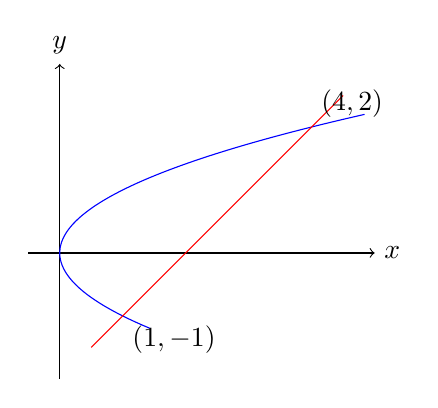
\begin{tikzpicture}[scale=0.8]
    \draw[->] (-0.5,0) -- (5,0) node[right] {$x$};
    \draw[->] (0,-2) -- (0,3) node[above] {$y$};
    \draw[domain=0:2.2, smooth, variable=\y, blue] plot ({\y^2}, {\y});
    \draw[domain=0:1.2, smooth, variable=\y, blue] plot ({\y^2}, {-\y});
    \draw[domain=0.5:4.5, smooth, variable=\x, red] plot ({\x}, {\x - 2});
    \node at (1,-1) [below right] {$(1,-1)$};
    \node at (4,2) [above right] {$(4,2)$};
\end{tikzpicture}
\end{center}
根据图像可以看出，如果先对 $y$ 积分，也就是从垂直$x$方向从下往上积分，那么积分区域 $D$ 势必被分成两部分，以$(1,-1)$为分界点．因此我们选择先对 $x$ 积分．对于每个固定的 $y$，$x$ 的积分限由两条曲线 $y^2 = x$ 和 $y = x - 2$ 决定．于是二重积分可以写成：
\[\iint_D xy \d \sigma = \int_{-1}^{2} \left( \int_{y^2}^{y+2} xy \d x \right) \d y \]
分别计算内层积分和外层积分：
\begin{align*}
\int_{-1}^{2} \left( \int_{y^2}^{y+2} xy \d x \right) \d y &= 
\int_{-1}^{2} y\d y\left[\frac{1}{2}x^2\right]_{y^2}^{y+2} \\
&=\frac{1}{2} \int_{-1}^{2} y\left( y^2 + 4y + 4 - y^4 \right) \d y \\
&=\frac{1}{2} \left[ -\frac{1}{6}y^6 + \frac{1}{4}y^4 + \frac{4}{3}y^3 +2y^2 \right]_{-1}^{2} \\
&=\frac{45}{8}
\end{align*}
\end{solution}
\begin{example}
    计算积分 $\int_0^1 x \d x \int_x^1 e^{-y^2} \d y$．
\end{example}
\begin{solution}
根据积分的上下限可以看出，积分区域$D$ 是由 $y = x$ 和 $y = 1$ 围成的区域．
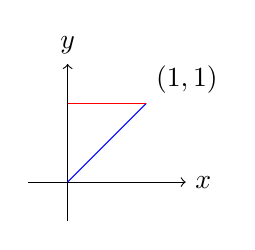
\begin{tikzpicture}
    \draw[->] (-0.5,0) -- (1.5,0) node[right] {$x$};
    \draw[->] (0,-0.5) -- (0,1.5) node[above] {$y$};
    \draw[domain=0:1, smooth, variable=\x, blue] plot ({\x}, {\x});
    \draw[domain=0:1, smooth, variable=\x, red] plot ({\x}, {1});
    \node at (1,1) [above right] {$(1,1)$};
\end{tikzpicture}
记积分结果为$I$，则交换积分顺序得到：
\begin{align*}
    I &= \int_0^1 e^{-y^2} \d y \int_0^y x \d x 
    = \frac{1}{3} \int_0^1 y^3 e^{-y^2} \d y 
    = \frac{1}{6} \int_0^1 y^2e^{-y^2} \d (y^2) 
    = -\frac{1}{6} \left[ (y^2 + 1)e^{-y^2} \right]_0^1 \\
    &= \frac{1}{6} - \frac{1}{3e}
\end{align*}
\end{solution}
\begin{example}
    计算积分 $\iint_D \max(xy,1) \d x \d y$，其中 $D = \{(x,y)|0 \le x \le 2, 0 \le y \le 2\}$．
\end{example}
\begin{solution}
根据函数 $\max(xy,1)$ 的定义，可以将积分区域 $D$ 分成两部分：\[
D_1 = \{(x,y)|0 \le x \le 2, 0 \le y \le 2, xy \le 1\} \quad \text{和} \quad D_2 = \{(x,y)|0 \le x \le 2, 0 \le y \le 2, xy > 1\}
\]记积分结果为$I$，则：\qquad\qquad\qquad\qquad\qquad\qquad\qquad\qquad\qquad\qquad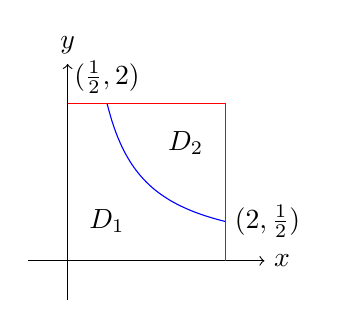
\begin{tikzpicture}
    \draw[->] (-0.5,0) -- (2.5,0) node[right] {$x$};
    \draw[->] (0,-0.5) -- (0,2.5) node[above] {$y$};
    \draw[domain=0.5:2, smooth, variable=\x, blue] plot ({\x}, {1/\x});
    \draw[domain=0:2, smooth, variable=\x, red] plot ({\x}, {2});
    \draw[domain=0:2, smooth, variable=\y, red] plot ({2}, {\y});
    \node at (1/2,2) [above] {$(\frac{1}{2},2)$};
    \node at (2,1/2) [right] {$(2,\frac{1}{2})$};
    \node at (0.5,0.5)  {$D_1$};
    \node at (1.5,1.5)  {$D_2$};
\end{tikzpicture}
\begin{align*}
    I &= \iint_{D_1} 1 \, \d x\d y+ \iint_{D_2} xy \, \d x\d y \\
    &= \int_\frac{1}{2}^2 x\d x \int_\frac{1}{x}^{2} y \, \d y + 4 -\int_\frac{1}{2}^2 \d x \int_\frac{1}{x}^2  \, \d y \\
    &= \int_{\frac{1}{2}}^{2} x\left(2-\frac{1}{2x^2} \right) \d x + 4 - \int_{\frac{1}{2}}^{2} \left( 2- \frac{1}{x} \right) \d x\\
    &= \left[ x^2 - \frac{1}{2} \ln x \right]_{\frac{1}{2}}^{2} + 4 - 3 + \ln x\Big|_{\frac{1}{2}}^{2} \\
    &= \frac{19}{4} + \ln 2
\end{align*}
\end{solution}
\section{三重积分}
\subsection{投影法}
\begin{theorem}
设 $D$ 是空间中的一个有界闭区域，$f(x,y,z)$ 在 $D$ 上连续．如果 $D$ 的投影区域 $D_{xy}$ 在 $xy$ 平面上是一个平面区域，并且对于每个 $(x,y) \in D_{xy}$，存在 $z_1(x,y)$ 和 $z_2(x,y)$ 使得 $(x,y,z) \in D$ 当且仅当 $z_1(x,y) \le z \le z_2(x,y)$，则三重积分 $\displaystyle\iiint_D f(x,y,z) \d V$ 可以表示为迭代积分：
\[\iiint_D f(x,y,z) \d V = \iint_{D_{xy}}\d x\d y\int_{z_1(x,y)}^{z_2(x,y)} f(x,y,z) \d z\]
\end{theorem}
\begin{example}
    计算积分 $\displaystyle\iiint_\Omega x \d V$，其中 $\Omega$ 为坐标面与平面 $x+2y+z=1$ 围成的区域．
\end{example}
\begin{solution}
首先确定积分区域 $\Omega$ 的边界．平面 $x+2y+z=1$ 与坐标面的交点可以通过解方程组
\[\begin{cases}
x + 2y + z = 1 \\
x = 0 \\
y = 0 \\
z = 0
\end{cases}\]
解得交点为 $(1,0,0)$、$(0,\frac{1}{2},0)$ 和 $(0,0,1)$．因此积分区域 $\Omega$ 是由坐标面和平面 $x+2y+z=1$ 围成的四面体．
于是有
\begin{align*}
    I &= \iiint_\Omega x \d V = \iint_{D_{xy}}x \d x\d y \int_0^{1-x-2y}  \d z = \iint_{D_{xy}} x(1-x-2y) \d x\d y \\
      &= \int_{0}^{1} x\d x \int_0^{\frac{1-x}{2}} (1-x-2y) \d y = \int_0^1 x\left[ (1-x)\cdot\frac{1-x}{2} - \left(\frac{1-x}{2}\right)^2\right] \d x\\
      &= \int_{0}^{1} x \cdot \frac{(1-x)^2}{4} \d x = \frac{1}{48}
\end{align*}
\end{solution}
\subsection{截面法}
\begin{theorem}
设 $\Omega$ 是空间中的一个有界闭区域，$f(x,y,z)$ 在 $\Omega$ 上连续．如果 $\Omega$ 在 $z$ 轴上的投影区间为 $[z_1, z_2]$，并且对于每个 $z \in [z_1, z_2]$，过点 $(0,0,z)$ 且垂直于 $z$ 轴的平面与 $\Omega$ 相交的平面区域为 $D_z$，则三重积分 $\displaystyle\iiint_\Omega f(x,y,z) \d V$ 可以表示为：
\[\iiint_\Omega f(x,y,z) \d V = \int_{z_1}^{z_2} \d z \iint_{D_z} f(x,y,z) \d x \d y\]
\end{theorem}
\begin{example}
    计算积分 $\displaystyle\iiint_\Omega z^2 \d V$，其中 $\Omega$ 是由椭球面 $\dfrac{x^2}{a^2}+\dfrac{y^2}{b^2}+\dfrac{z^2}{c^2}=1$ 围成的区域．
\end{example}
\begin{solution}
    积分区域 $\Omega$ 的形状如图所示：
    \begin{center}
    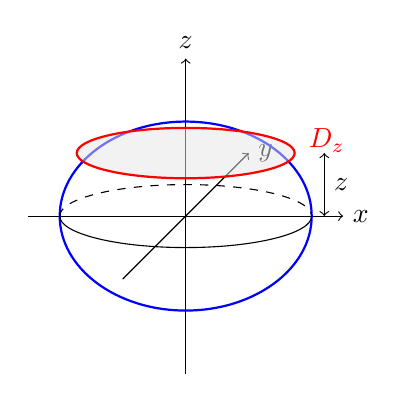
\begin{tikzpicture}[scale=0.8]
        \draw[->] (-2.5,0) -- (2.5,0) node[right] {$x$};
        \draw[->] (0,-2.5) -- (0,2.5) node[above] {$z$};
        \draw[->] (-1,-1) -- (1,1) node[right] {$y$};
        \draw[blue, thick] (0,0) circle [x radius=2, y radius=1.5];
        \draw[dashed] (-2,0) arc (180:0:2 and 0.5);
        \draw (2,0) arc (0:-180:2 and 0.5);
        \fill[gray!20, opacity=0.5] (0,1) ellipse (1.73 and 0.4);
        \draw[red, thick] (0,1) ellipse (1.73 and 0.4);
        \node at (1.8,1.2) [right, red] {$D_z$};
        \draw[<->] (2.2,0) -- (2.2,1) node[midway, right] {$z$};
    \end{tikzpicture}
    \end{center}
\[
        I = \int_{-c}^{c}z^2 \d z\iint_{D_z} \d x \d y
\]
注意到$D_z$为椭圆区域$\dfrac{x^2}{a^2(1-\frac{z^2}{c^2})}+\dfrac{y^2}{b^2(1-\frac{z^2}{c^2})}=1$，因此其面积为$\pi ab(1-\frac{z^2}{c^2})$．于是有
\[ I = \pi ab\int_{-c}^{c}(1-\frac{z^2}{c^2})z^2\d z = \frac{4}{15}\pi abc^3\]
\end{solution}
\begin{example}
    计算积分 $\displaystyle\iiint_\Omega z \d V$，其中 $\Omega$ 是抛物面 $z=x^2+y^2$ 与平面 $z=4$ 围成的区域．
\end{example}
\begin{solution}
    积分区域 $\Omega$ 的形状如图所示：
    \begin{center}
    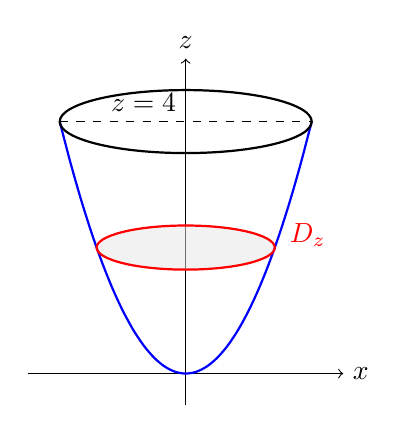
\begin{tikzpicture}[scale=0.8]
        \draw[->] (-2.5,0) -- (2.5,0) node[right] {$x$};
        \draw[->] (0,-0.5) -- (0,5) node[above] {$z$};
        \draw[domain=-2:2, smooth, variable=\x, blue, thick] plot ({\x}, {\x*\x});
        \draw[thick] (0,4) ellipse (2 and 0.5);
        \fill[gray!20, opacity=0.5] (0,2) ellipse (1.414 and 0.35);
        \draw[red, thick] (0,2) ellipse (1.414 and 0.35);
        \node at (1.5,2.2) [right, red] {$D_z$};
        \draw[dashed] (-2,4) -- (2,4);
        \node at (0,4) [above left] {$z=4$};
    \end{tikzpicture}
    \end{center}
    法一：投影法\\
    \[ I = \iint_{D_{xy}} \d x\d y \int_{x^2+y^2}^{4} z \d z = \iint_{D_{r\theta}} r\d r\d \theta \int_{r^2}^{4} z \d z = \pi \int_0^2 (16 - r^4)r \d r =  \frac{64}{3}\pi \]
    法二：截面法\\
    立体 $\Omega$ 在 $z$ 轴上的投影区间为 $[0, 4]$．对于任意固定的 $z \in [0, 4]$，水平面 $z$ 与 $\Omega$ 所截得的区域 $D_z$ 为圆区域：
    \[ D_z = \{(x,y) \mid x^2 + y^2 \le z\} \]
    其面积为 $S(z) = \pi (\sqrt{z})^2 = \pi z$．于是有：
    \[ I = \int_0^4 z \d z \iint_{D_z} \d x \d y = \int_0^4 z \cdot S(z) \d z = \int_0^4 \pi z^2 \d z = \frac{64\pi}{3} \]
\end{solution}
\section{重积分的对称性}
\subsection{普通对称性（奇偶性）}
\begin{theorem}
    函数的对称性往往可以简化积分的计算，具体来说：
    \begin{itemize}
        \item 若区域 $D$ (或 $\Omega$) 关于坐标面（或坐标轴）对称，而被积函数 $f$ 关于该对称变量为奇函数，则积分为 0．
        \item 若区域 $D$ (或 $\Omega$) 关于坐标面（或坐标轴）对称，而被积函数 $f$ 关于该对称变量为偶函数，则积分等于对称部分上积分的两倍．
    \end{itemize}
\end{theorem}

\begin{example}
    计算积分 $\iint_D e^{-x^2-y^2}-x^3e^y \d x \d y$，其中 $D$ 是以原点为中心，半径为 $a$ 的圆盘．
\end{example}
\begin{solution}
    \sout{圆神!启动！}\\
    换用极坐标，其中被积表达式中的第二项是关于$x$的奇函数，且区域 $D$ 关于 $y$ 轴对称，因此在圆盘$D$上积分为零．因此有
\[I = \iint_D e^{-x^2-y^2} \d x \d y = \int_0^{2\pi} \d \theta\int_0^a e^{-r^2}\cdot r \d r  = \pi (1 - e^{-a^2})\]
\end{solution}

\begin{example}
    设区域 $D$ 由 $y=4-x^2,y=-3x,x=1$ 围成，计算 $I=\iint_D y\ln(x+\sqrt{1+x^2})\d x \d y$．
\end{example}
\begin{solution}
首先确定积分区域 $D$ 的边界．曲线 $y=4-x^2$ 与 $y=-3x$ 的交点可以通过解方程组

\begin{tabular}{ll}
$\begin{cases}
y = 4 - x^2 \\
y = -3x
\end{cases}\quad\Rightarrow\qquad \begin{cases}
    (-1, 3) \\
    (4, -12)
\end{cases}$ & 
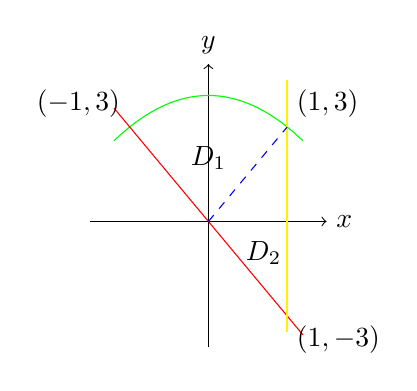
\begin{tikzpicture}[yscale=0.4, baseline=(current bounding box.center)]
    \draw[->] (-1.5,0) -- (1.5,0) node[right] {$x$};
    \draw[->] (0,-4) -- (0,5) node[above] {$y$};
    \draw[domain=-1.2:1.2, smooth, variable=\x, green] plot (\x, {4-\x*\x});
    \draw[domain=-1.2:1.2, smooth, variable=\x, red] plot (\x, {-3*\x});
    \draw[yellow, thick] (1,-3.5) -- (1,4.5);
    \draw[blue, dashed] (0,0) -- (1,3);
    \node at (-1,3) [above left] {$(-1,3)$};
    \node at (1,-3) [below right] {$(1,-3)$};
    \node at (1,3) [above right] {$(1,3)$};
    \node at (0,2)  {$D_1$};
    \node at (0.7,-1)  {$D_2$};
\end{tikzpicture}
\end{tabular}

其中$D_1$和$D_2$由直线 $y=3x$ 分开，于是二重积分可以写成：
\[ I=\iint_{D_1} y\ln(x+\sqrt{1+x^2})\d x \d y + \iint_{D_2} y\ln(x+\sqrt{1+x^2})\d x \d y\]
容易发现，$D_1$ 关于$y$轴对称，且被积函数是$x$的奇函数，因此$\iint_{D_1} y\ln(x+\sqrt{1+x^2})\d x \d y=0$．$D_2$ 关于$x$轴对称，且被积函数是$y$的奇函数，因此$\iint_{D_2} y\ln(x+\sqrt{1+x^2})\d x \d y=0$．综上所述，$I=0$．
\end{solution}

\subsection{轮换对称性}
\begin{theorem}[变量置换对称性]
    设积分区域 $\Omega \subset \mathbb{R}^n$ 为可求体积的集合．若存在变量的一置换 $\sigma \in S_n$，使得对于任意点 $\bm{x} = (x_1, \dots, x_n) \in \mathbb{R}^n$，满足 $\bm{x} \in \Omega$ 当且仅当 $\sigma(\bm{x}) = (x_{\sigma(1)}, \dots, x_{\sigma(n)}) \in \Omega$（即 $\Omega$ 在该置换下保持不变），则对于定义在 $\Omega$ 上的任何可积函数 $f$，有：
    \[ \int_{\Omega} f(x_1, \dots, x_n) \d V = \int_{\Omega} f(x_{\sigma(1)}, \dots, x_{\sigma(n)}) \d V \]
    特别地，若 $\Omega$ 在自变量的所有排列下均保持不变（完全轮换对称），则：
    \[ \int_{\Omega} f(x_1, \dots, x_n) \d V = \frac{1}{n!} \sum_{\sigma \in S_n} \int_{\Omega} f(x_{\sigma(1)}, \dots, x_{\sigma(n)}) \d V \]
    在三重积分的情形下，若 $\Omega$ 关于 $x, y, z$ 的轮换对称（如球面或立方体），则有：
    \[ \iiint_\Omega f(x,y,z) \d V = \iiint_\Omega f(y,z,x) \d V = \iiint_\Omega f(z,x,y) \d V \]
\end{theorem}

\begin{example}
    设区域 $D=\{(x,y) | x^2+y^2 \le 4,\; x,y \ge 0\}$，$f(x)$ 为$D$上正值连续函数，$a,b$为常数，求：
    \[I=\iint_D\frac{a\sqrt{f(x)}+b\sqrt{f(y)}}{\sqrt{f(x)}+\sqrt{f(y)}} \d \sigma \]
\end{example}
\begin{solution}
    注意到积分区域$D$关于$y=x$对称，且被积函数满足轮换对称，记$g(x,y)=\dfrac{a\sqrt{f(x)}+b\sqrt{f(y)}}{\sqrt{f(x)}+\sqrt{f(y)}}$，因此有
    \[ I = \frac{1}{2}\iint_D \left[ g(x,y) + g(y,x) \right] \d x \d y = \frac{1}{2}\iint_D (a+b) \d x \d y = \frac{a+b}{2}\pi\]
\end{solution}

\begin{example}
    计算积分$\displaystyle\iiint_\Omega z^2\d V$，其中$\Omega = \{(x,y,z) \mid x^2+y^2+z^2 \le 1\}$．
\end{example}
\begin{solution}
    由于积分区域$\Omega$关于 $x=y, y=z, z=x$ 面均对称，根据轮换对称性有
    \[ \iiint_\Omega x^2 \d V = \iiint_\Omega y^2 \d V = \iiint_\Omega z^2 \d V\]
    因此
    \[ I = \iiint_\Omega z^2\d V = \frac{1}{3}\iiint_\Omega (x^2+y^2+z^2) \d V\]
    利用球坐标计算（或直接利用体积结果）：
    \[ I = \frac{1}{3} \int_0^{2\pi} \d\phi \int_0^\pi \sin\theta \d\theta \int_0^1 r^2 \cdot r^2 \d r = \frac{1}{3} \cdot 4\pi \cdot \frac{1}{5} = \frac{4\pi}{15}\]
\end{solution}
\section{坐标变换与微元}

\subsection{坐标变换关系}
下表列出了常用的二维与三维坐标系之间的转换关系：
\begin{center}
\renewcommand{\arraystretch}{1.8}
\begin{tabular}{|c|l|l|}
\hline
\textbf{维度} & \textbf{变换类型} & \textbf{变量关系（正向与逆向）} \\ \hline
二维 & \textbf{直角} $(x,y) \leftrightarrow$ \textbf{极} $(r,\theta)$ & $\begin{cases} x = r\cos\theta \\ y = r\sin\theta \end{cases} \iff \begin{cases} r = \sqrt{x^2+y^2} \\ \theta = \arctan(\frac{y}{x}) \end{cases}$ \\ \hline \hline
\multirow{3}{*}{三维} & \textbf{直角} $(x,y,z) \leftrightarrow$ \textbf{柱} $(\rho,\phi,z)$ & $\begin{cases} x = \rho\cos\phi \\ y = \rho\sin\phi \\ z = z \end{cases} \iff \begin{cases} \rho = \sqrt{x^2+y^2} \\ \phi = \arctan(\frac{y}{x}) \\ z = z \end{cases}$ \\ \cline{2-3}
 & \textbf{直角} $(x,y,z) \leftrightarrow$ \textbf{球} $(r,\theta,\phi)$ & $\begin{cases} x = r\sin\theta\cos\phi \\ y = r\sin\theta\sin\phi \\ z = r\cos\theta \end{cases} \iff \begin{cases} r = \sqrt{x^2+y^2+z^2} \\ \theta = \arccos(\frac{z}{r}) \\ \phi = \arctan(\frac{y}{x}) \end{cases}$ \\ \cline{2-3}
 & \textbf{柱} $(\rho,\phi,z) \leftrightarrow$ \textbf{球} $(r,\theta,\phi)$ & $\begin{cases} \rho = r\sin\theta \\ \phi = \phi \\ z = r\cos\theta \end{cases} \iff \begin{cases} r = \sqrt{\rho^2+z^2} \\ \theta = \arctan(\frac{\rho}{z}) \\ \phi = \phi \end{cases}$ \\ \hline
\end{tabular}
\end{center}

\subsection{重积分变量替换公式（雅可比行列式）}
对于 $n$ 维变量替换 $\bm{x} = \bm{g}(\bm{u})$，其中 $\bm{u} = (u_1, u_2, \dots, u_n)$，重积分的变换公式为：
\[ \int_{\Omega} f(\bm{x}) \d V_x = \int_{\Omega'} f(\bm{g}(\bm{u})) \abs{ J } \d V_u \]
其中雅可比行列式（Jacobian Determinant）定义为：
\[ J = \frac{\partial(x_1, \dots, x_n)}{\partial(u_1, \dots, u_n)} = \det \begin{pmatrix}
    \pdv{x_1}{u_1} & \dots & \pdv{x_1}{u_n} \\
    \vdots & \ddots & \vdots \\
    \pdv{x_n}{u_1} & \dots & \pdv{x_n}{u_n}
\end{pmatrix} \]

\noindent \textbf{雅可比行列式的几何意义}：
\begin{itemize}
    \item \textbf{局部伸缩率}：$\abs{J}$ 描述了从 $\bm{u}$ 空间映射到 $\bm{x}$ 空间时，局部体积单元的\textbf{放大或缩小倍数}．
    \item \textbf{线性逼近}：在极小区域内，非线性变换 $\bm{g}$ 可以看作一个线性变换（由雅可比矩阵描述）．线性变换对体积的改变恰好是其变换矩阵的行列式．
    \item \textbf{示例（极坐标）}：在极坐标变换中，$J=r$．这意味着在原点附近（$r$ 很小），极大的角度变化也只对应很小的面积；而离开原点越远，同样的角度和半径增量所围成的面积越大．
\end{itemize}

\subsection{微元对照表}
在不同坐标系下，长度、面积、体积微元及雅可比行列式 $\abs{J}$ 的对应关系如下：

\noindent \textbf{1. 二维微元（极坐标变换）}
\begin{center}
\renewcommand{\arraystretch}{1.5}
\begin{tabular}{|c|c|c|c|}
\hline
\textbf{坐标系} & \textbf{线微元 $\d s^2$} & \textbf{面积微元 $\d \sigma$} & \textbf{雅可比 $\abs{J}$} \\ \hline
直角坐标 $(x,y)$ & $\d x^2 + \d y^2$ & $\d x \d y$ & 1 \\ \hline
极坐标 $(r,\theta)$ & $\d r^2 + r^2 \d \theta^2$ & $r \d r \d \theta$ & $r$ \\ \hline
\end{tabular}
\end{center}

\noindent \textbf{2. 三维微元（柱面与球面变换）}
\begin{center}
\renewcommand{\arraystretch}{1.6}
\begin{tabular}{|c|c|c|c|}
\hline
\textbf{坐标系} & \textbf{线微元 $\d s^2$} & \textbf{体积微元 $\d V$} & \textbf{雅可比 $\abs{J}$} \\ \hline
直角坐标 $(x,y,z)$ & $\d x^2 + \d y^2 + \d z^2$ & $\d x \d y \d z$ & 1 \\ \hline
柱面坐标 $(\rho,\phi,z)$ & $\d \rho^2 + \rho^2 \d \phi^2 + \d z^2$ & $\rho \d \rho \d \phi \d z$ & $\rho$ \\ \hline
球面坐标 $(r,\theta,\phi)$ & $\d r^2 + r^2 \d \theta^2 + r^2 \sin^2 \theta \d \phi^2$ & $r^2 \sin \theta \d r \d \theta \d \phi$ & $r^2 \sin \theta$ \\ \hline
\end{tabular}
\end{center}

\subsection{单位向量的微分与演化}
在正交曲线坐标系中，各点处的局部基向量（单位向量）通常随位置而改变．这种位置相关性在流体力学、动力学及张量分析中具有核心意义．

\noindent \textbf{1. 极坐标系下的单位向量微分}\\
基向量 $\bm{\hat{r}}$ 和 $\bm{\hat{\theta}}$ 定义为：
\[ \bm{\hat{r}} = \cos\theta \bm{i} + \sin\theta \bm{j}, \quad \bm{\hat{\theta}} = -\sin\theta \bm{i} + \cos\theta \bm{j} \]
其对坐标的演化关系如下：
\begin{center}
\renewcommand{\arraystretch}{1.5}
\begin{tabular}{|c|c|l|}
\hline
\textbf{算子} & \textbf{结果} & \textbf{几何直观/备注} \\ \hline
$\displaystyle\pdv{\bm{\hat{r}}}{\theta}$ & $\bm{\hat{\theta}}$ & $\bm{\hat{r}}$ 的转动速度为 $\bm{\hat{\theta}}$ \\ \hline
$\displaystyle\pdv{\bm{\hat{\theta}}}{\theta}$ & $-\bm{\hat{r}}$ & $\bm{\hat{\theta}}$ 的转动导致其指向中心 \\ \hline
$\displaystyle\pdv{\bm{\hat{r}}}{r}, \pdv{\bm{\hat{\theta}}}{r}$ & $\bm{0}$ & 单位向量方向与距离无关 \\ \hline
\end{tabular}
\end{center}

\noindent \textbf{2. 球坐标系下的单位向量微分}\\
定义 $\bm{\hat{r}}, \bm{\hat{\theta}}, \bm{\hat{\phi}}$ 为单位方向向量．它们的导数展现了复杂的耦合关系：
\begin{center}
\renewcommand{\arraystretch}{1.5}
\begin{tabular}{|c||c|c|c|}
\hline
\textbf{导数项} & $\bm{\hat{r}}$ & $\bm{\hat{\theta}}$ & $\bm{\hat{\phi}}$ \\ \hline\hline
$\displaystyle\pdv{}{\theta}$ & $\bm{\hat{\theta}}$ & $-\bm{\hat{r}}$ & $\bm{0}$ \\ \hline
$\displaystyle\pdv{}{\phi}$ & $\sin\theta \bm{\hat{\phi}}$ & $\cos\theta \bm{\hat{\phi}}$ & $-\sin\theta \bm{\hat{r}} - \cos\theta \bm{\hat{\theta}}$ \\ \hline
\end{tabular}
\end{center}
注：单位向量随 $\phi$ 的变化不仅依赖于 $\phi$ 方向本身，还受到天顶角 $\theta$ 的缩放因子控制．

\noindent \textbf{3. 位置向量的全微分与度规}\\
通过单位向量微分，位置向量 $\bm{r}$ 的全微分为：
\begin{itemize}
    \item \textbf{极坐标}：$\d\bm{r} = \d r \bm{\hat{r}} + r \d\theta \bm{\hat{\theta}}$
    \item \textbf{球坐标}：$\d\bm{r} = \d r \bm{\hat{r}} + r \d\theta \bm{\hat{\theta}} + r\sin\theta \d\phi \bm{\hat{\phi}}$
\end{itemize}
取模平方即可得到长度微元 $\d s^2 = \d\bm{r} \cdot \d\bm{r}$．
\section{重积分练习}
\begin{exercise}
    计算积分 $\displaystyle\iiint_\Omega (x+y+z^3) \d V$，其中 $\Omega$ 是由曲面$x^2+y^2+z^2=2z(z>1)$与$z=\sqrt{x^2+y^2}$所围成的区域．
\end{exercise}
\begin{solution}
根据对称性，由于积分区域 $\Omega$ 关于 $x=0$ 和 $y=0$ 平面对称，且 $x, y$ 均为奇函数，因此 $\iiint_\Omega x \d V = 0$ 和 $\iiint_\Omega y \d V = 0$．只需要计算 $\iiint_\Omega z^3 \d V$．

采用球坐标系更为简便．曲面 $x^2+y^2+z^2=2z$ 即 $\rho = 2\cos\phi$．条件 $z>1$ 实际上对应于球面的上半部分，它与下方的圆锥面 $z=\sqrt{x^2+y^2}$ (即 $\phi = \frac{\pi}{4}$) 正好在 $z=1$ 处相交．因此区域 $\Omega$ 在球坐标下可表示为：
\[ \Omega = \{ (\rho, \theta, \phi) \mid 0 \le \theta \le 2\pi, \quad 0 \le \phi \le \frac{\pi}{4}, \quad 0 \le \rho \le 2\cos\phi \} \]
体积微元 $\d V = \rho^2\sin\phi \d\rho\d\phi\d\theta$．代入得：
\begin{align*}
\iiint_\Omega z^3 \d V &= \int_0^{2\pi} \d\theta \int_0^{\frac{\pi}{4}} \d\phi \int_0^{2\cos\phi} (\rho\cos\phi)^3 \rho^2\sin\phi \d\rho \\
&= 2\pi \int_0^{\frac{\pi}{4}} \cos^3\phi \sin\phi \left[ \frac{\rho^6}{6} \right]_0^{2\cos\phi} \d\phi \\
&= 2\pi \int_0^{\frac{\pi}{4}} \frac{32}{3}\cos^9\phi \sin\phi \d\phi \\
&= \frac{64\pi}{3} \left[ -\frac{\cos^{10}\phi}{10} \right]_0^{\frac{\pi}{4}} 
= \frac{32\pi}{15} \left( 1 - \frac{1}{32} \right) = \frac{31\pi}{15}
\end{align*}
\end{solution}

\begin{exercise}
    $\Sigma_1$是以点$(0,4,0)$为顶点且与曲面$\Sigma_2: \dfrac{x^2}{3}+\dfrac{y^2}{4}+\dfrac{z^2}{3}=1(y>0)$相切的圆锥面，求$\Sigma_1$与$\Sigma_2$所围成的区域的体积．
\end{exercise}
\begin{solution}
作变量代换：令 $u = \frac{x}{\sqrt{3}}, v = \frac{y}{2}, w = \frac{z}{\sqrt{3}}$，在此变换下，雅可比行列式 $J = \sqrt{3} \times 2 \times \sqrt{3} = 6$．

在 $uvw$ 空间中，$\Sigma_2$ 变为了单位上半球面 $u^2+v^2+w^2=1 (v>0)$，圆锥顶点变为了 $(0,2,0)$．
图形具有旋转对称性，可使用柱坐标系（以 $v$ 轴为中心轴，极径 $r = \sqrt{u^2+w^2}$）．
过顶点 $(0,2)$ 作单位圆 $r^2+v^2=1$ 的切线．设切线方程为 $r = k(2-v)$，代入圆方程得 $(k^2+1)v^2 - 4k^2v + 4k^2-1 = 0$．根据相切条件判别式 $\Delta=0$ 解得 $k = \frac{1}{\sqrt{3}}$，对应的切点高度为 $v = \frac{1}{2}$．

所以，在新空间中该区域的体积 $V'$ 可由一个圆锥的体积减去一个球冠的体积得到：
\begin{itemize}
    \item \textbf{圆锥体积}（顶点 $v=2$，底面在 $v=\frac{1}{2}$ 处，底面半径 $r=\frac{\sqrt{3}}{2}$）：
    \[ V_{cone} = \frac{1}{3}\pi \left(\frac{\sqrt{3}}{2}\right)^2 \times \left(2 - \frac{1}{2}\right) = \frac{3\pi}{8} \]
    \item \textbf{球冠体积}（$v$ 从 $\frac{1}{2}$ 到 $1$）：
    \[ V_{cap} = \int_{\frac{1}{2}}^1 \pi(1-v^2) \d v = \pi \left[ v - \frac{v^3}{3} \right]_{\frac{1}{2}}^1 = \frac{5\pi}{24} \]
\end{itemize}
使得 $V' = \frac{3\pi}{8} - \frac{5\pi}{24} = \frac{\pi}{6}$．
原体积 $V = \iiint_\Omega \d x\d y\d z = 6 \iiint_{\Omega'} \d u\d v\d w = 6 V' = \pi$．
\end{solution}

\begin{exercise}
    计算积分 $\displaystyle\iiint_\Omega \dfrac{xyz}{x^2+y^2}\d V$，其中 $\Omega$ 是曲面 $(x^2+y^2+z^2)^2=2a^2xy\ (a>0)$ 的第一象限部分． 
\end{exercise} 
\begin{solution}
采用球坐标系（取 $x=r\sin\theta\cos\phi, y=r\sin\theta\sin\phi, z=r\cos\theta$），第一象限对应 $0 \le \theta \le \frac{\pi}{2}$，且 $0 \le \phi \le \frac{\pi}{2}$．

代入曲面方程，得区域 $\Omega$ 的边界：
\[ r^4 = 2a^2(r\sin\theta\cos\phi)(r\sin\theta\sin\phi) \implies r^2 = a^2\sin^2\theta\sin(2\phi) \]
故极径的积分范围为 $0 \le r \le a\sin\theta\sqrt{\sin(2\phi)}$．

体积微元 $\d V = r^2\sin\theta \d r\d\theta\d\phi$．被积函数为：
\[ \frac{xyz}{x^2+y^2} = \frac{(r\sin\theta\cos\phi)(r\sin\theta\sin\phi)(r\cos\theta)}{r^2\sin^2\theta} = r\cos\theta\sin\phi\cos\phi \]
将积分转化为累次积分：
\begin{align*}
    I &= \int_0^{\frac{\pi}{2}} \d\phi \int_0^{\frac{\pi}{2}} \d\theta \int_0^{a\sin\theta\sqrt{\sin(2\phi)}} (r\cos\theta\sin\phi\cos\phi)(r^2\sin\theta) \d r \\
      &= \int_0^{\frac{\pi}{2}} \d\phi \int_0^{\frac{\pi}{2}} \sin\theta\cos\theta\sin\phi\cos\phi \left[ \frac{r^4}{4} \right]_0^{a\sin\theta\sqrt{\sin(2\phi)}} \d\theta \\
      &= \frac{a^4}{4} \int_0^{\frac{\pi}{2}} \d\phi \int_0^{\frac{\pi}{2}} \sin\theta\cos\theta\sin\phi\cos\phi \left( \sin^4\theta \cdot 4\sin^2\phi\cos^2\phi \right) \d\theta \\
      &= a^4 \int_0^{\frac{\pi}{2}} \sin^5\theta\cos\theta \d\theta \int_0^{\frac{\pi}{2}} \sin^3\phi\cos^3\phi \d\phi
\end{align*}
分别计算这两个单变量积分：
\[ \int_0^{\frac{\pi}{2}} \sin^5\theta\cos\theta \d\theta = \left[ \frac{1}{6}\sin^6\theta \right]_0^{\frac{\pi}{2}} = \frac{1}{6} \]
\[ \int_0^{\frac{\pi}{2}} \sin^3\phi\cos^3\phi \d\phi = \int_0^{\frac{\pi}{2}} \sin^3\phi (1-\sin^2\phi) \d(\sin\phi) = \frac{1}{4} - \frac{1}{6} = \frac{1}{12} \]
最终结果为：
\[ I = a^4 \times \frac{1}{6} \times \frac{1}{12} = \frac{a^4}{72} \]
\end{solution}

\begin{exercise}
    设 $\Omega$ 是由平面 $\Pi_1:x=0, \Pi_2:x=y, \Pi_3:y=z, \Pi_4:z=1, \Pi_5:z=2$ 所围成的空间区域，求三重积分 $\displaystyle\iiint_\Omega \frac{\d x\d y\d z}{\sqrt{y^2+z^2}}$．
\end{exercise}
\begin{solution}
由题目给出的各个平面方程式可以推断出，积分区域 $\Omega$ 的上下限关系为：
\[ 1 \le z \le 2, \quad 0 \le y \le z, \quad 0 \le x \le y \]
利用累次积分（先对 $x$ 积分，再对 $y$ 积分，最后对 $z$ 积分）得：
\begin{align*}
    I &= \int_1^2 \d z \int_0^z \d y \int_0^y \frac{1}{\sqrt{y^2+z^2}} \d x \\
      &= \int_1^2 \d z \int_0^z \frac{y}{\sqrt{y^2+z^2}} \d y \\
      &= \int_1^2 \left[ \sqrt{y^2+z^2} \right]_{y=0}^{y=z} \d z \\
      &= \int_1^2 (\sqrt{2z^2} - \sqrt{z^2}) \d z \\
      &= \int_1^2 (\sqrt{2}-1)z \d z = (\sqrt{2}-1) \left[ \frac{z^2}{2} \right]_1^2 = \frac{3(\sqrt{2}-1)}{2}
\end{align*}
\end{solution}
\ifx\allfiles\undefined
\end{document}
\fi